\newpage
\section{Bola, Para Bola}           

We've mentioned several times that a parabola is the set of points
that are equidistant from a given point (the focus) and a given line
(the directrix):\index{focus}\index{directrix}
\[
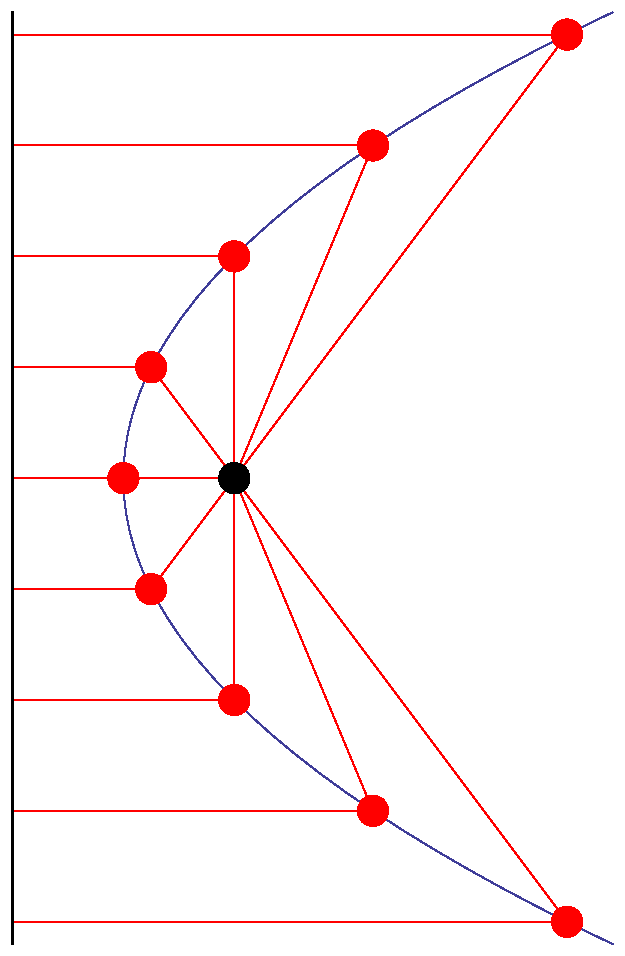
\includegraphics[angle=90,scale=.4]{../graphics/parabolapointline.pdf}
\]
In this activity we are going to try an reconcile the definition given
above with the equation that you know and love (admit it!):
\[
y = ax^2 + bx + c
\]

\begin{prob}
How do we compute the distance between two points? Be explicit!
\end{prob}

\begin{prob}
Let's see if we can derive the formula for a parabola with its focus at $(0,1)$ and its directrix being the line $y=0$.
\begin{enumerate}
\item Given a point $(x,y)$, write an expression for the distance from this point to the focus.
\item Write an expression for the distance from $(x,y)$ to the directrix. 
\item Use these two expressions and some algebra to find the formula for the parabola. 
\end{enumerate}
\end{prob}

\begin{prob}
Let's see if we can derive the formula for a parabola with its focus at $(0,1)$ and its directrix being the line $y=-1$.
\begin{enumerate}
\item Given a point $(x,y)$, write an expression for the distance from this point to the focus.
\item Write an expression for the distance from $(x,y)$ to the directrix. 
\item Use these two expressions and some algebra to find the formula for the parabola. 
\end{enumerate}
\end{prob}


\begin{prob}
Let's see if we can derive the formula for a parabola with its focus at $(1,1)$ and its directrix being the line $y=-2$.
\begin{enumerate}
\item Given a point $(x,y)$, write an expression for the distance from this point to the focus.
\item Write an expression for the distance from $(x,y)$ to the directrix. 
\item Use these two expressions and some algebra to find the formula for the parabola. 
\end{enumerate}
\end{prob}



